\documentclass{beamer}
\usepackage[utf8]{inputenc}
\usepackage[czech]{babel}
\usepackage[IL2]{fontenc}
\usepackage{newcent}
\usepackage{graphicx}
\usetheme{Berkeley}
\setbeamertemplate{logo}{ITY 5. projekt}
\usepackage{booktabs}

\begin{document}
	\begin{frame}
		\title{Konečné automaty}
		\subtitle{Typografie a publikování - 5. projekt}
		\author{Tomáš Nereča}
		\institute{Vysoké učení technické v~Brně\\
			Fakulta informačních technologií}
		\maketitle
	\end{frame}
	
	\begin{frame}
		\frametitle{Obsah}
		\tableofcontents
	\end{frame}

	\section{Formální definice}
	\begin{frame}
		\frametitle{Formální definice}
		Konečný automat (KA) je pětice:
		$M = (Q, \Sigma, R, s, F)$, kde:
		\begin{itemize}
			\item $Q$ je konečná množina stavů
			\item $\Sigma$ je vstupní abeceda
			\item $R$ je konečná množina pravidel tvaru: $pa\rightarrow q$,
			kde $p, q \in Q, a \in \Sigma \cup \{\varepsilon\}$
			\item $s \in Q$ je počáteční stav
			\item $F \subseteq Q$ je množina koncových stavů
		\end{itemize}
	\end{frame}

	\section{Popis činnosti KA}
	\begin{frame}
		\frametitle{Popis činnosti KA}
		\begin{itemize}
			\item Automat v počátečním stavu
			\item Opakované čtení symbolů a přechod do dalšího stavu dle přechodové tabulky
			\item Pokud automat skončí ve stavu z množiny přijímajících stavů, automat vstup přijal
			\item V opačném případe automat vstup nepřijal
		\end{itemize}
	\end{frame}

	\section{Grafické znázornění KA}
	\begin{frame}
		\frametitle{Grafické znázornění KA}
		Obvykle se používá grafické znázornění, na kterém kolečka znázorňují jednotlivé stavy a šipky (s přidruženým vstupním symbolem) mezi těmito kolečky popisují jednotlivé přechody.
		
		Příklad takového znázornění pro předchozí ukázkový automat je na obrázku:\\
		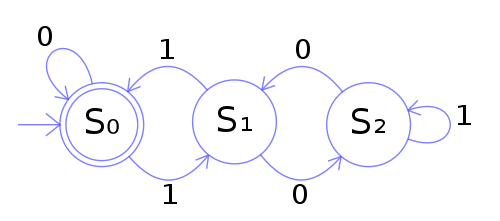
\includegraphics[height=4cm]{example.png}
	\end{frame}

	\section{Formalizace výpočtu KA}
	\begin{frame}
		\frametitle{Formalizace výpočtu KA}
		\begin{block}{Konfigurace KA}
			Konfigurace KA je dvojice $(q , w) \in K \times \Sigma^*$, kde $q$ je aktuálny stav automatu a $w$ je doposud neprečtená část vstupného slova.
		\end{block}
		\begin{block}{Krok výpočtu KA}
			Krokem výpočtu KA je relace $\vdash_A$ na konfiguracích KA definovaná nasledovne: $(q, av) \vdash_A (p, v) \Longleftrightarrow p = \delta (q, a)$.
		\end{block}
		\begin{block}{Jazyk akceptovaný pomocí KA}
			Jazyk akceptovaný KA $A$ definujeme nasledovne:
			$L(A) = \{w \mid \exists p\in F:(q_0, w) \vdash_A^*(p, \varepsilon)\}.$
		\end{block}
	\end{frame}
\end{document}